\documentclass{beamer}
\usepackage{../common_slides}
\usepackage{tikz-qtree}

\title{Language Modeling \\ + \\ Feed-Forward Networks 3}
\date{}
\author{Alexander Rush}

\usepackage{stackengine}
\stackMath
\newlength\matfield
\newlength\tmplength
\def\matscale{1.}
\newcommand\dimbox[3]{%
  \setlength\matfield{\matscale\baselineskip}%
  \setbox0=\hbox{\vphantom{X}\smash{#3}}%
  \setlength{\tmplength}{#1\matfield-\ht0-\dp0}%
  \fboxrule=1pt\fboxsep=-\fboxrule\relax%
  \fbox{\makebox[#2\matfield]{\addstackgap[.5\tmplength]{\box0}}}%
}
\newcommand\raiserows[2]{%
   \setlength\matfield{\matscale\baselineskip}%
   \raisebox{#1\matfield}{#2}%
}
\newcommand\matbox[4]{
  \stackunder{\dimbox{#1}{#2}{$#4$}}{\scriptstyle #3}%
}

\begin{document}

\begin{frame}
  \titlepage
\end{frame}

\begin{frame}{Review: Machine Learning Setup}

  Multi-class prediction problem, 

  \[ (\boldx_1, \boldy_1), \ldots, (\boldx_n, \boldy_n) \]
  \begin{itemize}
  \item $\boldy_i$; the one-hot next word
  \item $\boldx_i$; representation of the prefix $(w_1, \ldots, w_{t-1})$
  \end{itemize}
  \pause
  \textbf{Challenges:}
  \begin{itemize}
  \item How do you represent input?
  \item Smoothing is crucially important.
  \item Output space is very large (next class)
  \end{itemize}
\end{frame}

\begin{frame}{Review: Perplexity}
  Previously, used \textit{accuracy} as a metric.
  
  \air 

  Language modeling uses of version  average negative
  log-likelihood 
  \begin{itemize}
    \item For test data $\bar{w}_1, \ldots, \bar{w}_n$
    \item \[NLL = -\frac{1}{n}\sum_{i=1}^n \log p(w_i | w_1, \ldots,w_{i-1})\]
  \end{itemize}


  Actually report \textit{perplexity},
  \[ perp = \exp(-\frac{1}{n}\sum_{i=1}^n \log p(w_i | w_1, \ldots,w_{i-1})) \]

  Requires modeling full distribution as opposed to argmax (hinge-loss)
\end{frame}

\begin{frame}{Idea 1: Interpolation (Jelinek-Mercer Smoothing)}
  Can write recursively,

  \[ p_{interp}(w |  c) =  \lambda p_{ML}(w |  c) + (1 - \lambda) p_{interp}(w | c') \]

  Ensure that $\lambda$ form convex combination
  \[0 \leq \lambda \leq 1\]

  How do you learn conjunction combinations?
\end{frame}


\begin{frame}{Quiz}
  We talked briefly last class about using language models for smoothing. 
  It has become a popular task in recent years to utilize language models to predict 
  missing words, for example consider the Microsoft Research Sentence Completion Challenge.

  \begin{center}
    a tractor rode slow

    a red tractor rode fast

    the parrot flew fast

    the parrot flew slow
    
    the tractor slowed down


    the  red \_\_\_ ?

    the  red \_\_\_ flew fast?
  \end{center}

\end{frame}



\begin{frame}
  %   \begin{tabular}{lll}
  %     the & red & 0.5\\
  %     the & blue & 0.5\\
  %     red & tractor &   0.8\\ 
  %     red & parrot &   0.2\\
  %     parrot & flew &   0.9 \\
  %     tractor & flew &   0.1 \\
  %     flew & high &   0.6 \\
  %     flew & low &   0.4 \\
  %   \end{tabular}
  % \end{center}
\end{frame}


\begin{frame}{Today's Class }
  \[ p(w_i | w_{i-n+1}, \ldots w_{i-1}; \theta) \] 

  \begin{itemize}
  \item Estimate this directly as a neural network.
    \air 

  \item Two types of models, neural network and bilinear. 
    \air 

  \item Efficiency methods for estimation.
  \end{itemize}
\end{frame}


\begin{frame}{Intuition: NGram Issues}
  
  In training we see, 

  \begin{center}
    the arizona corporations commission \alert{authorized}
  \end{center}

  But at test we see, 
  \begin{center}
    the colorado businesses organization \alert{\_\_\_}
  \end{center}
  \pause 
  
  \begin{itemize}
  \item Does this training example help here?
    \begin{itemize}
    \item Not really. No count overlap.
    \end{itemize}
    \air 
  \item Does backoff help here? 
    \begin{itemize}
    \item Maybe, if we have seen organization.
    \item Mostly get nothing from the earlier words.
    \end{itemize}
  \end{itemize}
\end{frame}


\begin{frame}{Class-Based Language Models}
  
\end{frame}

\section{Neural Language Models}

\begin{frame}{Recall: Word Embeddings}
  \begin{itemize}
  \item Embeddings allow us to utilize similar words
  \end{itemize}

  arizona
  \begin{tabular}{ll}
  texas& 0.932968706025 \\
  florida & 0.932696958878\\
  kansas&0.914805968271\\
  colorado&0.904197441085\\
  minnesota&0.863925347525\\
  carolina&0.862697751337\\
  utah& 0.861915722889\\
  miami&0.842350326527\\
  oregon&0.842065064748\\
  \end{tabular}

  corporations
  \begin{tabular}{ll}
  firms& 0.894882639809\\
  companies&0.86738377358\\
  businesses&0.859315950927\\
  corporate&0.821590295322\\
  enterprises&0.818504805202\\
  investing&0.765133327454\\
  institutions&0.76372338938\\
  subsidiaries&0.762939166391\\
  lobbyists&0.759909805468\\
  \end{tabular}
\end{frame}

\begin{frame}{Issues}

  Although... in training we see, 

  \begin{center}
    the eagles play the arizona \alert{diamondbacks}
  \end{center}

  And at test we might see, 

  \begin{center}
    the eagles play the colorado  \alert{}
  \end{center}  
\end{frame}

\begin{frame}{Feed-Forward Neural NNLM (Bengio, 2003)}
  \begin{itemize}
  \item $\boldx$ is an embedded representation
  \end{itemize}
\end{frame}


\begin{frame}{Feed-Forward Neural Representation}
  \begin{itemize}
  \item $p(w_i | w_{i-n+1}, \ldots w_{i-1}; \btheta)$
  \item $f_1, \ldots, f_{\dwin}$ are words in window
  \item Input representation is the concatenation of embeddings
  \end{itemize}

  \[ \boldx = [v(f_1)\  v(f_2) \  \ldots \  v(f_{\dwin})]  \]

  Example: Tagging
  \[ [\textcolor{blue}{w_3\ w_4\ w_5\ w_6\ w_7}]\ \textcolor{red}{w_8} \]
  \[ \boldx = [v(w_3)\  v(w_4) \  v(w_5) \ v(w_6) \ v(w_7)]  \]

  \[\renewcommand\matscale{.6}
\matbox{1.5}{4}{\din /5}{} \matbox{1.5}{4}{\din /5}{} \matbox{1.5}{4}{\din /5}{\boldx} \matbox{1.5}{4}{\din /5}{} \matbox{1.5}{4}{\din /5}{}% \raiserows{1.5}{\matbox{4}{2}{d_0}{\dout}{\boldW^0}}  \matbox{4}{2}{\din}{\dout}{\boldW^1} +
% \matbox{7}{2}{1}{\dout}{\boldb}
\]

  
\end{frame}


\begin{frame}{A Neural Probabilistic Language Model (Bengio, 2003)}  
  One hidden layer multi-layer perceptron architecture,

  \[NN_{MLP1}(\boldx) =  \tanh(\boldx\boldW^1 + \boldb^1)W^2 + \boldb^2\]
  
  Neural network architecture on top of concat.

  \[\hat{\boldy} = \softmax(NN_{MLP1}(\boldx)) \] 
\end{frame}

\begin{frame}{A Neural Probabilistic Language Model }  
  Optional, direct connection layers,

  \[NN_{DMLP1}(\boldx) =  [\tanh(\boldx\boldW^1 + \boldb^1), \boldx] W^2 + \boldb^2\]

  \begin{itemize}
  \item $\boldW^1 \in \reals^{\din \times \dhid}, \boldb^1 \in \reals^{1 \times \dhid}$; first affine transformation
  \item $\boldW^2 \in \reals^{(\dhid + \din)  \times \dout}, \boldb^2 \in \reals^{1 \times \dout}$; second affine transformation
  \end{itemize}
\end{frame}

\begin{frame}{A Neural Probabilistic Language Model (Bengio, 2003)}  
  \begin{center}
    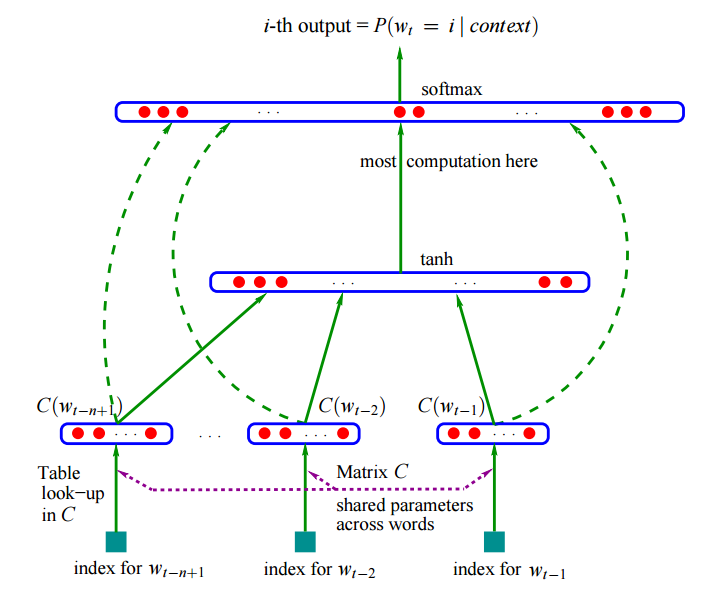
\includegraphics[width=7cm]{bengio}
  \end{center}
\end{frame}



\begin{frame}{A Neural Probabilistic Language Model (Bengio, 2003)}  
  \begin{center}
    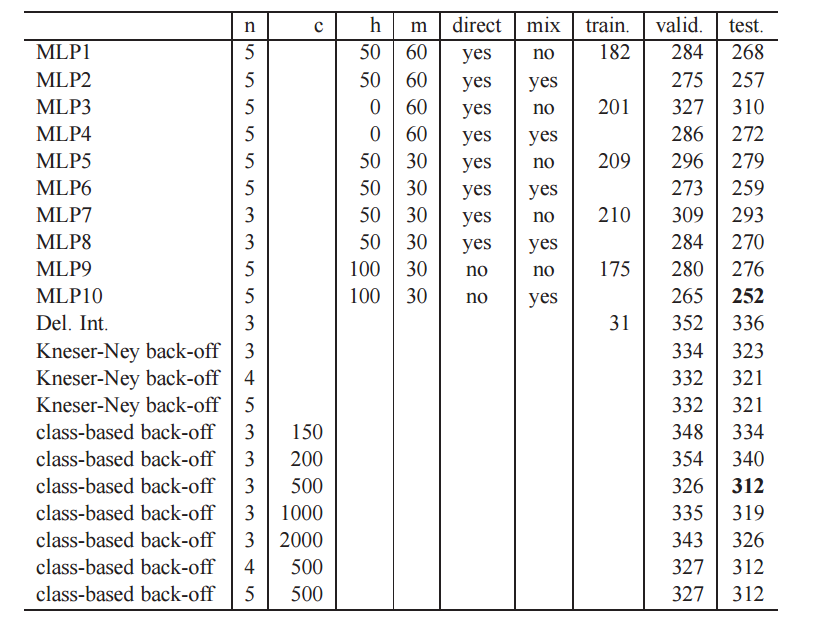
\includegraphics[width=7cm]{bengioresults}
  \end{center}
\end{frame}

\begin{frame}{Parameters}
  \begin{itemize}
  \item Bengio NNLM has $\dhid=100$, $\dwin=5$, $\din = 5 \times 50 $ 
    \air 
    
  \item In-Class: How many parameters does it have? How does this compare to Kneser-Ney smoothing?
  \end{itemize}

\end{frame}


\begin{frame}{Log-Bilinear Language Model ()}

  \[\hat{\boldy} = \softmax((\boldx)\boldW^1 + \boldb)\]

  \begin{itemize}
  \item Remove the tanh layer, but maintain ordering.
    \air 

  \item Dense $\boldx$ concatenated word-embeddings
  \end{itemize}
\end{frame}



\begin{frame}{Neural Language Modeling}
  NGram Models
  \begin{itemize}
  \item Fast to train 
  \end{itemize}

  Neural Models
  \begin{itemize}
  \item Make Markov assumption
  \item Slower to train
  \item
  \end{itemize}
\end{frame}

\begin{frame}{NGram Models}
  
\end{frame}

\section{Noise Contrastive Estimation}

\begin{frame}{Review: Softmax Issues}
  Use a softmax to force a distribution,

  \[\softmax(\boldz) = \frac{\exp(\boldz)}{\displaystyle \sum_{c\in \mcC } \exp(z_c)}  \]

  \[\log \softmax(\boldz) = \boldz - \log \sum_{c\in \mcC} \exp(z_c)  \]

  \begin{itemize}
  \item \textbf{Issue:} class $\mcC$ is huge.
  \item For C\&W, 100,000, for word2vec 1,000,000 types
  \item Note largest dataset is 6 billion words
  \end{itemize}

\end{frame}



\begin{frame}{Unnormalized Network}
  Recall the score defined as, 
  \[ \boldz = \tanh(\boldx \boldW^1)\boldW^2 + \boldb \] 

  Unnormalized score of each word. 

  \[ z_i = \tanh(\boldx \boldW^1)\boldW^2_{*,i} + b_i \] 

  Can be computed efficiently $O(1)$ versus $O(|\mcV|)$. 
\end{frame}


\begin{frame}{Coherence Estimation }
  \begin{itemize}
  \item \textbf{Idea:} Learn to distinguish coherent n-grams from 
    corruption. 
    \air 
 
  \item Similar idea to ranking embedding, but no score function. 

  \item Want to differentiate,

    \begin{center}
      [ the dog \structure{walks} ]
    \end{center}
    
    
    
    It should score higher than,
    \begin {center}
      [ the dog \alert{house}  ]
      
      [ the dog \alert{cats}  ]
      
      [ the dog \alert{skips}  ]
      
    \end{center}
  \end{itemize}
\end{frame}

\begin{frame}{}
  Imagine we had this dataset 
  \[ (\boldx_1, \boldy_1),\ldots, (\boldx_n, \boldy_n), \]
  
  Where $\boldy$ was 

  \[ \mathcal{L}(\theta) = \sum_{i} L_{cross}(\boldy, \hat{\boldy}) \] 

\end{frame}

\begin{frame}{Recall: Binary Classification}
  \[ \mathcal{L}(\theta) = \sum_{} L_{cross}() \]   
\end{frame}



\begin{frame}{NCE 1}
  Random variable $D$

  $D=1$ with prob $\frac{1}{K+1}$

  $D=0$ with prob $\frac{K}{K+1}$
  
  If $D=1$ then generate a true word, otherwise if $D=0$ generate from noise distribution. 
\end{frame}

\begin{frame}
  \[P(D=1 | \boldx, \boldy) =  \frac{P(X|D, Y) P(X| Y)}{\sum_{d} P(X|D) P(X) } =  \frac{P(X|D) P(X)}{P(X|D)P(x) +  P(X|D) P(x) }\] 

  \[  \frac{1/{k+1} p(X)}{1/{k+1} p(X) + (k)/(k+1) P(n_i) } = \frac{p(X)}{p(X) + (k) P(n_i) } \]

  \[ \sigma(z_w - \log(k P(w))) \]
\end{frame}


\begin{frame}{NCE 2}
  \[ \mathcal{L}(\theta) = \sum_{i} \log P(D=1| X_i, Y) + \sum_{k=1}^{K} P(D=0|X_i, = )  \] 
  
  \[ \mathcal{L}(\theta) = \sum_{i} \log \sigma(z_w - \log(k P(w)))  + \sum_{k=1}^{K} (1- \sigma(z_w - \log(k P(w))))  \] 
\end{frame}

\begin{frame}{Implementation}
  How do you efficiently compute $z_w$? 

  Need a lookup table for output embeddings! (not linear) and dot product.

  How do you efficiently handle $p(w)$ 
  
  Also can be done with lookuptable and add.

  How do you handle sampling? 

  Can precompute large number of samples (not example specific).

  How do you handle loss?

  Simply BinaryNLL Objective.
\end{frame}

\begin{frame}{Implementation}
  
  Standard MLP language model,

  \[\boldx \Rightarrow \boldW^1 \Rightarrow \tanh \Rightarrow  \boldW^2 \Rightarrow \softmax\]



  Computing $\sigma(z_w - \log(k P(w)))$,
 \[\boldx \Rightarrow \boldW^1 \Rightarrow \tanh \Rightarrow
 \begin{matrix}
   \cdot \\ 
   \boldW^2_{*, w} \mathrm{(Lookup)}
 \end{matrix}
 \Rightarrow  \begin{matrix}
   - \\ 
   K p(w) \mathrm{(Lookup)}
 \end{matrix}
\Rightarrow \sigma\]


 %  $\boldx$ $\Rightarrow$ linear $\Rightarrow$ tanh  $\Rightarrow$\begin{tabular}{l} Dotproduct & LookupTable ($W_{}$)\end{tabular}
 % $\Rightarrow $ \begin{tabular}{l} Add \\ LookupTable (P(w))\end{tabular} $\Rightarrow$ Sigma
 
                                                                                       
  % \Tree [ .LookupTable [ .Linear [ .tanh [ .DotProduct(with w) [ .Subtract (log P(w))  .Sigma ]     ]  ]  ] ] ;   

  (Efficiency, compute first three layers only once for $K+1$)

\end{frame}


\begin{frame}{Noise Distribution}
  What noise distribution should you use.

  Unigram estimations.
\end{frame}


\begin{frame}{Use as an LM}
  \begin{itemize}
  \item Unlike HSM learns full $\boldW^2$ 
    \air 

  \item Can run $\softmax(tanh(\boldx \boldW^1) + \boldW^2)$ at test time. 

  \item Instead of 1 multiclass, we do 1+K binary classifications


  \end{itemize}
\end{frame}

% \% begin{frame}{Comparison With }
%   \begin{itemize}
%   \item 
%   \item 
%   \end{itemize}
% \end{frame}

% \begin{frame}{Loss Criterions}

%   \begin{center}

%   \begin{tikzpicture}
%     \node(x)[text width=3cm,text centered]{prediction\\ $\hat{\boldY} $};
%     \node(t)[text  width=3cm,text centered, below right= of x, draw]{  $L(*, *)$};

%     \node(fx)[text width=3cm,text centered, above right=of t]{loss\\$L(\boldY, \hat{\boldY})$};
%     \node(gradin)[text width=3cm,text centered, below left =of t]{self.gradInput\\ $\displaystyle \frac{\partial L}{\partial \hat{\boldY} } $};
%     \node(gradout)[text width=3cm,text centered, below right= of t]{target \\ $\boldY$   };
%     % \node(gradweight)[text width=3cm,text centered, below = of t]{self.gradWeight\\ $\displaystyle  \frac{\partial L}{\partial \btheta_{i+1}  }$};

%     \path[text width=3cm,text centered, draw, ->] (x) -> (t);
%     \path[text width=3cm,text centered, draw, ->] (t) -> (fx);
%     \path[text width=3cm,text centered, draw, ->] (t) -> (gradin);
%     \path[text width=3cm,text centered, draw, ->]  (gradout) -> (t);
%   \end{tikzpicture}
%   \end{center}
% \end{frame}


\end{document}